\subsection{Some Detections of LIGO}

\subsubsection{GW190814}

Two advanced-LIGO detectors (Hanford, Washington and Livingston, Louisiana, USA) and the advanced-Virgo detector (Cascina, Italy), have detected gravitational waves from the inspiral and merger of a stellar-mass black hole and another compact object on 14th August, 2019 at 21:10:39 UTC. It has been named as GW190814 as the date suggests.

\begin{figure}[h]
    \centering
    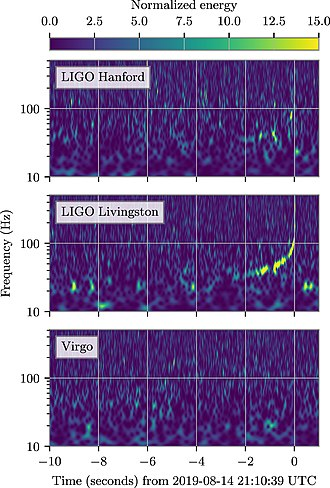
\includegraphics[scale = 0.91]{images.tex/GW190814.jpg}
    \caption{Frequency Vs Time data of GW190814 in three observatories. Source:- \href{https://en.wikipedia.org/wiki/GW190814}{Wikipedia}}
\end{figure}

While the mass of one component of this binary could range from 22.2 to 24.3 $M_\odot$ black hole, the other component which was of 2.6 solar mass could be either a low-mass black hole or a heavy neutron star. The masses of the objects before merging differed by a factor of 9. This makes it the most extreme mass ratio known for some GW event. The source of this GW was in a small patch of sky of around 20 square degrees. Even after doing so much research, the counterpart of the black hole which was in the inspiral mechanism wasn’t observed. It can be that, either black hole consumed the neutron star completely or both were black holes. Had we observe an electromagnetic counterpart, which may not have happened due to a number of reasons, we could say the smaller object is mostly neutron star. 

\pagebreak

\subsection{GW170817}

On 17th August, 2017, LIGO and Virgo detectors observed a gravitational wave named as GW170817. It is known to be produced by two neutron stars merging into each other while spiralling closer and closer. The aftermath of this GW was observed by around 70 observatories on 7 continents as well as through space, across the electromagnetic spectrum, marking a significant breakthrough for multi-messenger astronomy. The discovery and subsequent observations of GW170817 got Breakthrough of the Year award for 2017 by the journal Science.

\begin{figure}[h]
    \centering
    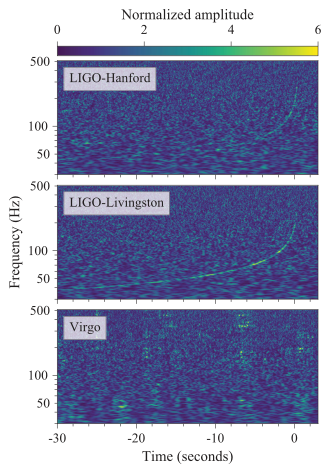
\includegraphics[scale=0.78]{images.tex/GW170817_observatories.png}
    \caption{Frequency Vs Time data of GW170817 in three observatories. Source:- \href{https://en.wikipedia.org/wiki/GW170817}{Wikipedia}}
\end{figure}

The component masses of the binary are inferred to be between 1.17 and 1.60 $M_\odot$. After merging it makes the mass of about 2.74 $M_\odot$. The gravitational wave signal lasted for about 100 seconds. It started with a frequency of 24 $Hz$. It  inspiralled for around 3,000 cycles. The amplitude and frequency increased to a few hundred hertz as both the objects came nearer in the typical inspiral chirp pattern. Lastly, it ended with the collision at 12:41:04.4 UTC which was received as a signal in the interferometer. At first, it arrived at the Virgo detector in Italy. After 22 milliseconds, detectors at the LIGO-Livingston detector in Louisiana, United States got the signals. After another 3 milliseconds, the waves reached at the LIGO-Hanford detector in the state of Washington, United States. It was then compared with a prediction from the general theory of relativity given by Einstein to analyse it further. The source was localised within a sky region of 28\degree square which has a probability of 90\%.

A gamma-ray burst, GRB 170817A was detected. It lasted for $\approx$ 2 seconds. It was detected by Fermi and INTEGRAL spacecrafts. This bursts began at 1.7 seconds after the signal received denoting the merge of the objects. It's a hypothesis that neutron star mergers cause gamma-ray bursts which gets confirmed with this merger.





\pagebreak
